\section{Temperature Box}
\label{sec:temperature_box}

Even though previous setups used an infrared lamp~\cite{Boano2013, Hermans2013} to heat the motes directly, we chose to control mote temperature sorely using air temperature.
The mote is placed in a closed styrofoam box and the confined air is heated to the requested temperature and circulated to transfer this heat to the mote.

\subsection{Hardware}
A microcontroller evaluates temperature sensors within the box and locally controls the duty cycles of a small fan and 150W ceramic heating element using a PID loop to achieve the requested air temperature.
The microcontroller can communicate over a serial connection to receive the desired temperature and send the current temperature.

Additionally, air temperature is displayed as a hue from blue (cold) via green (warm) to red (hot) on a RGB LED.
The duty cycles of the heating element and fan are mapped to two white LEDs, to provide an immidiate status overview and prevent burn injuries.

The box is powered by a 300W PC power supply, which was chosen for its ability to provide 12V, 5V and 3.3V at the required currents, which removes the need for additional (costly) voltage conversion.
A custom designed PCB distibutes power from the ATX connectors to two high and two medium power MOSFET switches and up to five temperature sensors, all controlled by an ATmega328p.

The PCB, heating element and fan are fixed on a wooden baseplate using fasteners and screws.
All custom made parts were prototyped using the PCB mill and lasercutter of the RWTH FabLab~\cite{fablab}.
The styrofoam box has the outside dimensions of $35 \times 35 \times 30$cm with a wall thickness of 5cm which results in a holding capacity of $12.5\ell$.

Picture~\ref{pic:box_hardware} shows the controller, heating element, fan and mote harness.

\subsection{Embedded Software}

The embedded software is written using the xpcc microcontroller framework~\cite{xpcc.io} and implemented as a set of asynchronous control tasks for input parsing and output formatting, temperature sensor evaluation, PID loop update and duty cycle generation.
All switching frequencies were kept well below 1kHz to avoid any kind of interference with the 2.4GHz band.

\subsection{Performance}

The heating element has enough power to heat the air inside the box up to $120\,^{\circ}\mathrm{C}$.
This can however damage both the styrofoam material as well as the mote, so a limit of $90\,^{\circ}\mathrm{C}$ is imposed during experiments.

As seen in Figure~\ref{fig:box_heating_cooling} it takes about 40 minutes to heat up to $90\,^{\circ}\mathrm{C}$ and about 2 hours to cool back down to $30\,^{\circ}\mathrm{C}$.
The PID loop is deliberately dampened so that no overshoot in air temperature occurs, however, since the mote temperature naturally lags behind, a slight overshoot in air temperature might actually help achieve desired mote temperature quicker.
However, during the experiments a more granular approach is used similar to Figure~\ref{fig:box_heating_step}.

With a room temperature of $20-25\,^{\circ}\mathrm{C}$, the minimum experiment temperature was set at $30\,^{\circ}\mathrm{C}$ so that it can be reached within reasonable time.
The boxes can be retrofitted with an active piezoelectric cooling element and a fan by connecting them to the two unused MOSFET switches on the controller and updating the software.

\begin{figure}[H]
	\centering
    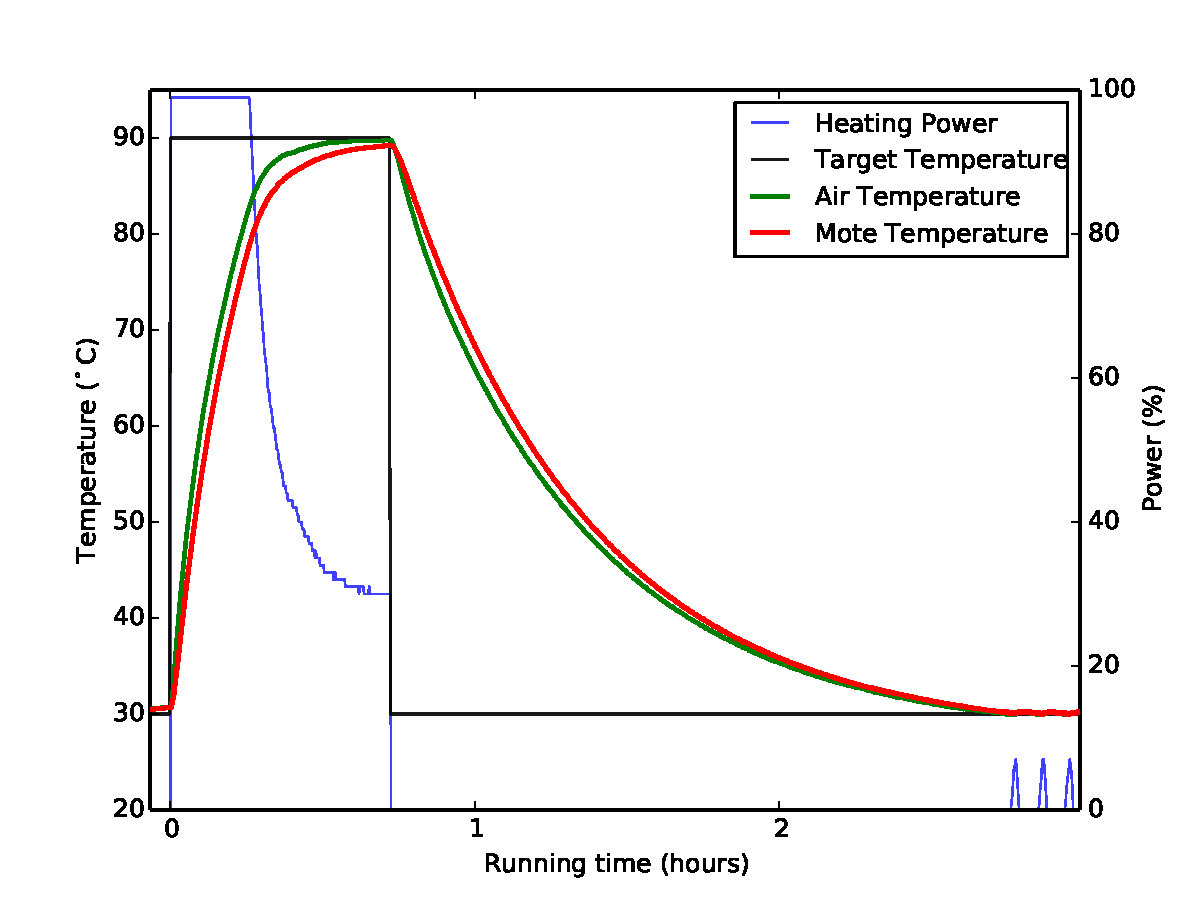
\includegraphics[width=1\columnwidth]{figures/box_heating_cooling}
	\caption{Temperature box heating up to $90\,^{\circ}\mathrm{C}$, then cooling back down to $30\,^{\circ}\mathrm{C}$.}
    \label{fig:box_heating_cooling}
\end{figure}

\begin{figure}[H]
	\centering
    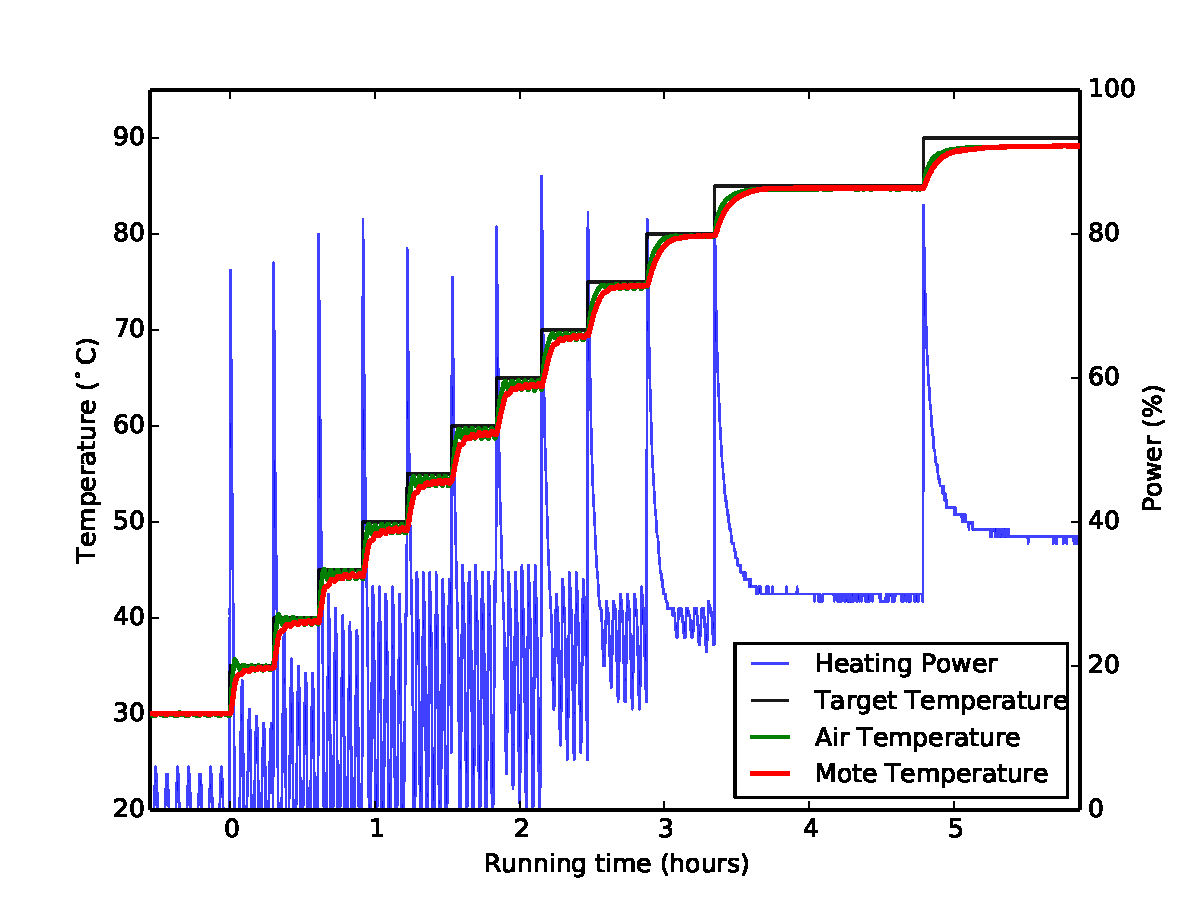
\includegraphics[width=1\columnwidth]{figures/box_heating_step}
	\caption{Example experiment run with temperature increments of $5\,^{\circ}\mathrm{C}$.}
    \label{fig:box_heating_step}
\end{figure} 